

\documentclass[twocolumn]{article}

\usepackage{indentfirst}
\usepackage{float}
\setlength{\parindent}{2em}

\usepackage{graphicx}
\graphicspath{ {images/} }

\usepackage[linesnumbered,ruled,vlined]{algorithm2e}

\usepackage{amsmath}
\usepackage[margin=1cm]{geometry}

\usepackage{biblatex}

\bibliography{s.bib}



\title{Parallel approach to single-source shortest path problem\\ on large complete graphs}

\author{Ruijian An}

\begin{document}
\date{}
\maketitle

\section{Introduction}
The single-source shortest path (SSSP) problem is a fundamental part of graph theory, with applications in transportation theory, road networks, DNA micro-arrays and many others. Given a weighted graph \emph{G = (V, E)} and a source vertex \emph{v}, the SSSP problem computes the shortest paths from \emph{v} to all other vertices. 

There are many efficient sequential solutions to this problem, such as Dijkstra's algorithm and the Bellman-Ford algorithm\cite{corman}. To maximize the work efficiency, Dijkstra's algorithm, which runs in \emph{O($|E| + |V|log|V|$)}, utilizes a greedy strategy, processing vertices one by one. On the other hand, the Bellman-Ford algorithm, which runs in O(\emph{$|E||V|$}), processes all vertices in every stage. Nevertheless, for large complete graphs, these sequential algorithms take a prohibitive amount of time for time-sensitive applications.

Although Dijkstra's algorithm is sequential in nature, the Bellman-Ford algorithm contains a lot of parallelism which can be exploited to speed up the processing of large graphs. Our goal is to parallelize the latter algorithm, by utilizing the massively parallel architecture of Graphics Processing Units(GPUs) on large complete graphs. By efficiently implementing the algorithm on a GPU, our implementation gains a speedup of 167x over the naive parallel GPU version and 10.6x over the optimized parallel CPU version for large graphs with up to 20000 vertices.

\section{Background}
\subsection{The Bellman-Ford algorithm}
\begin{algorithm}
\SetAlgoLined
\KwIn{G, w, s}
$s.d = 0$\;
\For{each vertex $v \in G.V$} {
  v.d = INFINITY\;
}
\For{$i \gets 1$ \textbf{to} $\left|G.V\right| - 1$}{
    \For{each edge $(u, v) \in G.E$}{
    RELAX(u, v, w)\;
    }
}
 \caption{BELLMAN\_FORD}
\end{algorithm}

\begin{algorithm}
\SetAlgoLined
$v.d = min(v.d, u.d + w(u, v))$\;
\caption{RELAX}
\end{algorithm}
In the Bellman-Ford algorithm, each vertex in the graph has an attribute \emph{d}, which records the tentative distance from source vertex to itself. The algorithm also employs a technique called \emph{relaxation} to process edges. If an edge (\emph{u,v}) with weight \emph{w(u,v)} is relaxed, \emph{v.d} is replaced by \emph{min(v.d, u.d + w(u,v))}. The Bellman-Ford algorithm relaxes each edge for $\left|V\right|$ - 1 times, resulting in a time complexity of O($\left|V\right|$$\left|E\right|$).

\subsection{GPU programming model}

NVIDIA's CUDA is a user-friendly compute framework for carrying out general-purpose computations on GPUs\cite{nvi}. A CUDA program contains a kernel function, which is executed on the GPU, using a user-specified number of threads. All threads in a kernel have a unique ID, such that the kernel can assign different work based on the thread IDs. A typical CUDA program consists of three parts: copying the input data to GPU memory, launching a kernel which performs computations on the data and transferring data back to CPU memory. The data transfer time between CPU and GPU memory is typically a scalability bottleneck.


\section{Approach}
Our goal is to exploit the inherent data parallelism from the Bellman-Ford algorithm and accelerate it using parallelization techniques. First, we implement a straightforward naive parallelization, both on the CPU and on the GPU. Next, we optimize both implementations by improving work efficiency. Finally, we leverage GPU-specific features and mitigate the overheads of transferring data between main memory and device memory.

The straightforward naive parallelization takes advantage of the inherent data parallelism. First, the shortest path estimate can be initialized in parallel. Secondly, edge relaxation, the most expensive step in the algorithm, can be parallelized. In existing parallel Bellman-Ford algorithms, each thread gets assigned a set of vertices and is responsible for relaxing either all the incoming or outgoing edges from its vertices\cite{Busato2016AnEI}\cite{Harish2007}. This approach uses adjacency lists and is well-suited for sparse graphs where $|V|$ is much larger than $|E|$. We use this as our naive multithreaded CPU implementation and naive GPU implementation. 

We observe that for complete graphs, partitioning work based on edges instead of vertices can exploit a higher degree of parallelism. While this approach is not straightforward to implement on the CPU, GPUs provide the ability to structure computations in a two-dimensional grid, where partitioning work by edges comes naturally. We use this observation as the baseline for our optimized GPU implementation and employ an adjacency matrix representation to better enable parallel edge relaxation on the GPU in an efficient manner.

Next, we implement the optimized versions of the parallel CPU and GPU algorithms, which provide better work efficiency. We take advantage of two techniques, to discard unnecessary work. In the basic algorithm, all edges are required to be relaxed in each iteration, but not all relaxations are useful. For edge \emph{(u, v)}, the key of \emph{relaxation} is to compare \emph{v.d} with \emph{u.d + w(u,v)}, so the relaxation is useful only if the \emph{v.d} is updated in the previous iteration. Otherwise, the relaxation of \emph{(u, v)} involves redundant work. In the improved implementation, a bit \emph{mask} is used to record whether vertices are active. If a vertex's attribute \emph{d} is modified, then the corresponding bit indicates it is an active vertex. In the subsequent iterations, only edges whose starting vertex is active will be relaxed. 

Building on our previous observation, we can also reduce the number of iterations that the basic algorithm executes ($|V|-1$). The program can terminate once all shortest path distances converge, so instead of stopping at $|V|$-1, we can terminate early in an iteration when there are no more active vertices. We maintain a \emph{flag} to indicate if any vertices are active during the current iteration, and once the flag becomes unset, we skip the remaining iterations and terminate the execution early.


Finally, a serialization bottleneck in our naive GPU implementation is the data transfer to device memory. In the optimized GPU algorithm, we restructure the code to leverage streams, which enable pipelining data transfers with computations.
We create two streams \emph{(stream1, stream2)} and partition the adjacency matrix equally between them. Each part of the matrix is transferred to the device and processes in a different stream. Consequently, computations on the first part of the matrix can be carried out concurrently with transferring the second part of the matrix to the device, thus reducing the transfer time in half. We can further reduce this by similarly using more streams.



\section{Analysis}
We conduct two sets of experiments (using randomly-generated complete graphs): first, we compare a
sequential CPU implementation, a naive multithreaded CPU version (by doing edge relaxation in parallel over 4 physical cores on a Core i7 6700HQ @ 2.6Ghz), and a naive GPU-based algorithm(on an NVIDIA Geforce GTX750 Ti, 640 cores, @ 1100MHz), all of which are unoptimized. The second graph compares the optimized multithreaded CPU implementation with the optimized GPU algorithm as described in Section 3. We include the basic (unoptimized) \textit{parallel} CPU and GPU implementations as a reference point in the second graph. Both optimized versions enforce the aforementioned work efficiency optimizations, and the latter also leverages GPU streams for overlapping data transfers with computations.\newline
\begin{figure}[h]

\centering
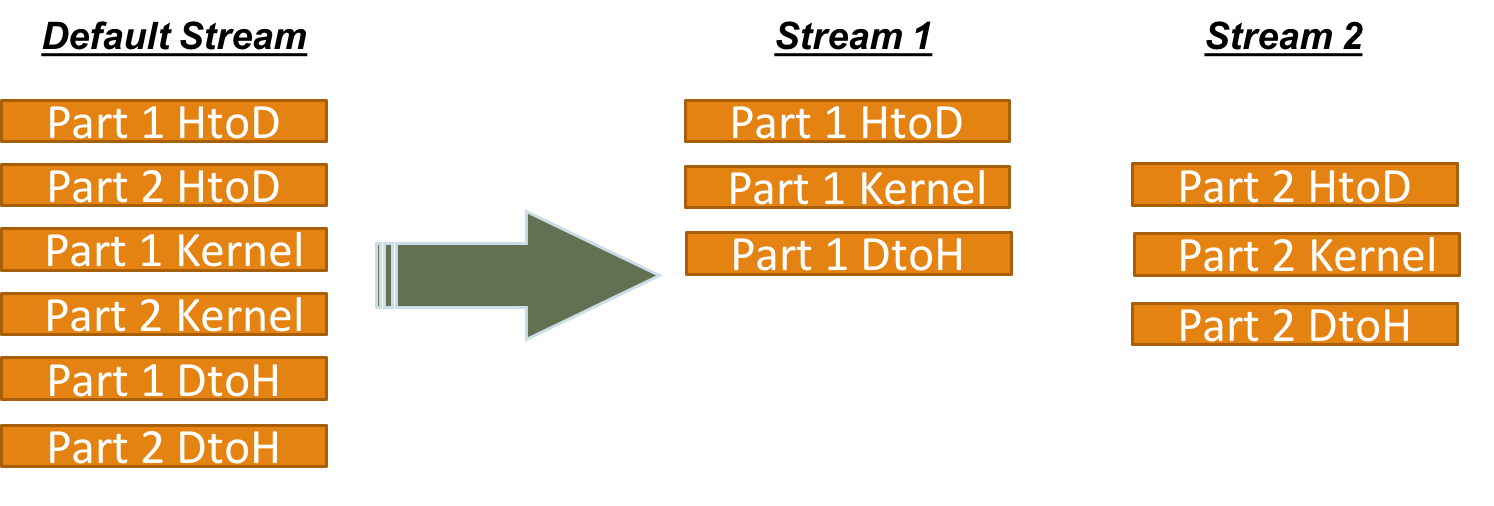
\includegraphics[width=0.45\textwidth]{fig1}
\caption{Straightforward (work inefficient) parallelization on the CPU and GPU (log scale on y axis)}
\end{figure}


\begin{figure}[h]

\centering
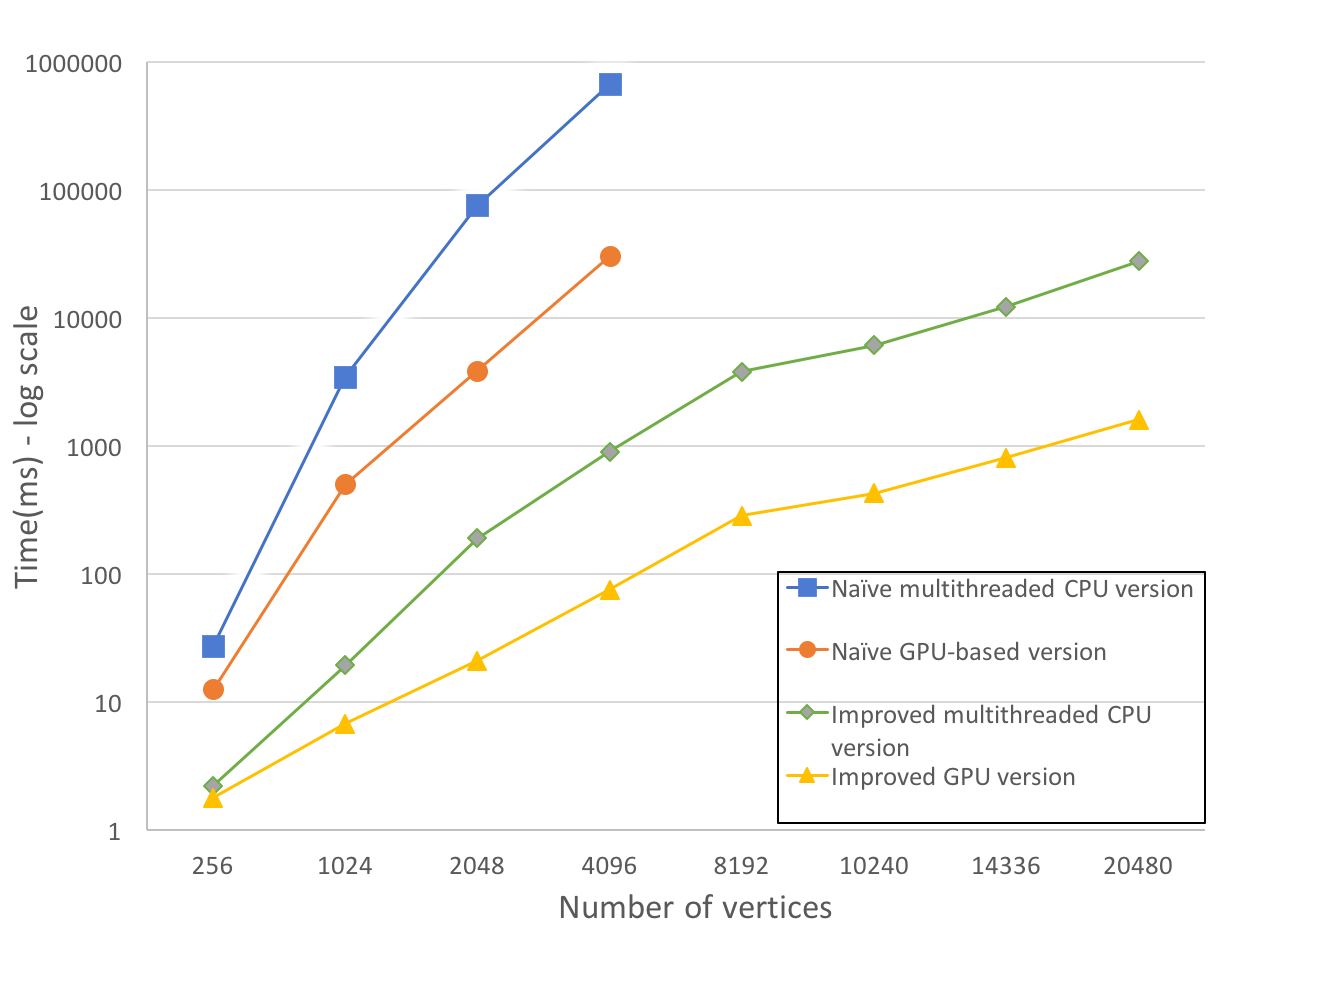
\includegraphics[width=0.5\textwidth]{fig2}
\caption{Work ineffcient vs. optimized algorithm implementations (log scale on y axis)}
\label{ab}
\end{figure}
In the first comparison, the naive GPU implementation outperforms both sequential CPU and naive multithreaded CPU versions. All implementations perform unnecessary computations, and the GPU implementation also suffers from high data transfer overheads to device memory. Consequently, we restructure parallel algorithms to reduce work inefficiencies, and use GPU streams to overlap memory transfers.

Our results from Figure 2 show that the optimized GPU algorithm outperforms its optimized CPU counterpart, achieving a 10.6x speedup for a large graph with 20000 vertices. When the graph is small, the difference between the two implementations is not significant because only a subset of GPU cores are utilized and CPU cores operate at a much higher clock rate. However, the gap increases with input size, as more GPU cores actively participate in computations, while the same number of CPU cores process increasingly larger tasks. Although our testing limitations did not permit testing with larger graphs (e.g., millions of vertices), we expect this gap will increase even further.

The optimizations and use of streams in the GPU implementation reduce the execution time by 167x compared to the work inefficient GPU version, while the optimized CPU implementation achieves up to 334x speedup over the work inefficient multithreaded CPU implementation, on large graphs.

\section{Conclusion}
Our work proposes an improved parallel Bellman-Ford algorithm implementation. By reworking the algorithm to leverage GPU-specific optimizations, reduce work inefficiencies, and deal with the data transfer overheads using streams, the proposed implementation is 167x faster than a naive GPU implementation, and 10.6x faster than an optimized parallel CPU implementation, on large graphs.

\printbibliography

\end{document}